
\mySection{L’Apprentissage Profond et ses Limites}{}
L’apprentissage profond (\textit{deep learning}, DL) a révolutionné de nombreux domaines grâce à sa capacité à modéliser des relations complexes dans des données volumineuses et non structurées. Cette section vise à établir les bases théoriques du DL, en explorant ses principes fondamentaux, ses applications dans des domaines critiques comme le contrôle d’accès, et les limites inhérentes à son opacité, qui freinent son adoption dans des systèmes où la transparence est essentielle \cite{jouis2020}. L’objectif est de fournir un cadre conceptuel pour comprendre pourquoi l’explicabilité est cruciale pour surmonter ces défis, en particulier dans le contexte de la cybersécurité et de la gestion des accès \cite{zhang2022xai}.

\mySubSection{Introduction à l’Apprentissage Profond}{}
L’apprentissage profond est une sous-discipline de l’apprentissage automatique qui repose sur des réseaux de neurones artificiels organisés en couches multiples, capables de traiter des données complexes sans nécessiter d’ingénierie manuelle des caractéristiques \cite{lecun2015deep}. Apparu comme une approche dominante dans les années 2010, le DL a permis des avancées majeures dans des domaines variés, tels que la reconnaissance d’images, le traitement du langage naturel, et la cybersécurité. Dans le contexte du contrôle d’accès, les modèles de DL sont de plus en plus utilisés pour détecter des anomalies, gérer des permissions dynamiques, et auditer les accès \cite{nobi2022dlbac}. Cette sous-section introduit les concepts clés du DL, met en lumière ses avantages (par exemple, l’extraction automatique de caractéristiques, la robustesse face à des données hétérogènes), et souligne son rôle croissant dans les systèmes critiques où la précision et l’adaptabilité sont primordiales \cite{barredo2020xai}.

\begin{figure}[h]
    \centering
    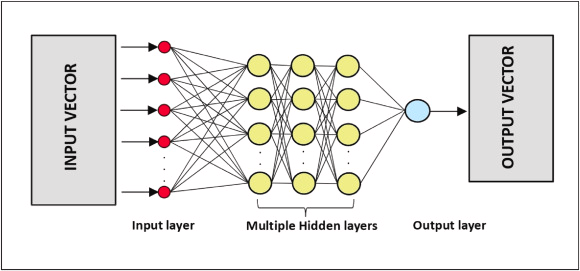
\includegraphics[width=0.8\textwidth]{My-Thesis/Chap1/images/deep_learning_model.png}
    \caption{Représentation schématique d’un réseau de neurones profond, illustrant les couches d’entrée, cachées, et de sortie, ainsi que le flux de données à travers les connexions pondérées. Cette visualisation montre la complexité des architectures de DL, qui contribue à leur puissance mais aussi à leur opacité.}
    \label{fig:dl_overview}
\end{figure}

\mySubSection{Principes Fondamentaux du Deep Learning}{}
\mySubSubSection{Architecture des Réseaux de Neurones}{}
Les réseaux de neurones profonds sont composés de multiples couches de neurones artificiels, interconnectés par des poids appris lors de l’entraînement. Chaque neurone effectue une transformation linéaire suivie d’une fonction d’activation non linéaire (par exemple, ReLU, sigmoïde), permettant au réseau de modéliser des relations complexes \cite{lecun2015deep}. Les architectures courantes incluent les réseaux convolutifs (CNN) pour les données structurées, les réseaux récurrents (RNN) pour les séquences, et les réseaux à attention pour les tâches nécessitant une focalisation sur des éléments spécifiques. Dans le contrôle d’accès, les CNN peuvent analyser des logs formatés, tandis que les RNN sont adaptés à l’analyse des historiques d’accès \cite{karpathy2015visualizing}. Cette sous-section détaille la structure des réseaux, leur modularité, et leur capacité à s’adapter à différents types de données.

\begin{figure}[h]
    \centering
    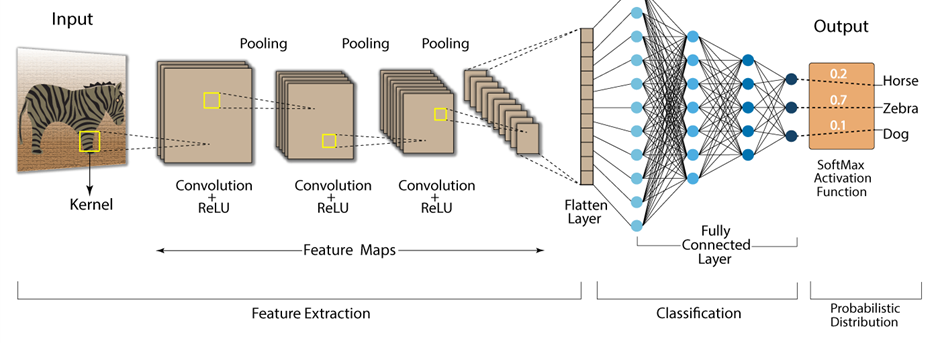
\includegraphics[width=1.0\textwidth]{My-Thesis/Chap1/images/cnn.png}
    \caption{Architecture d’un réseau convolutif (CNN), montrant les couches de convolution, de pooling, et de classification. Cette visualisation illustre comment un CNN extrait des caractéristiques hiérarchiques à partir de données.}
    \label{fig:cnn_architecture}
\end{figure}

\mySubSubSection{Processus d’Entraînement}{}
L’entraînement d’un modèle de DL repose sur la minimisation d’une fonction de perte, qui mesure l’écart entre les prédictions du modèle et les valeurs attendues. Ce processus utilise la rétropropagation du gradient pour ajuster les poids des connexions, souvent via des algorithmes d’optimisation comme la descente de gradient stochastique (SGD) ou Adam \cite{lecun2015deep}. Cette sous-section explique les étapes clés de l’entraînement, les besoins en données volumineuses et étiquetées, et les défis liés à la qualité des données, comme les biais ou les données incomplètes, qui peuvent affecter les performances dans le contrôle d’accès \cite{slack2020fooling}. Elle aborde également l’importance des hyperparamètres (taux d’apprentissage, taille des couches) et des ressources computationnelles nécessaires.

\mySubSubSection{Types de Modèles de Deep Learning}{}
Cette sous-section présente les modèles de DL les plus pertinents pour le contrôle d’accès :
\begin{itemize}
    \item \textbf{Réseaux Convolutifs (CNN)} : Utilisés pour traiter des données structurées, comme les images ou les logs d’accès formatés. Les CNN extraient des motifs spatiaux, utiles pour détecter des anomalies dans les métadonnées d’accès \cite{selvaraju2017gradcam}.
    \item \textbf{Réseaux Récurrents (RNN) et LSTM} : Conçus pour les données séquentielles, comme les historiques d’accès, permettant de modéliser des comportements temporels \cite{karpathy2015visualizing}.
    \item \textbf{Réseaux à Attention} : Ces modèles, comme les transformers, mettent en évidence les attributs critiques (par exemple, localisation ou heure) dans les décisions d’accès \cite{lin2017structured}.
\end{itemize}
Chaque type est illustré par son application potentielle dans le contrôle d’accès, avec un accent sur leur adaptabilité aux environnements dynamiques.

\mySubSection{Applications du Deep Learning dans le Contrôle d’Accès}{}
Le DL offre des solutions puissantes pour moderniser les systèmes de contrôle d’accès, surpassant souvent les approches traditionnelles comme le \textit{Role-Based Access Control} (RBAC) ou l’\textit{Attribute-Based Access Control} (ABAC) \cite{sandhu1996role, hu2013abac}. Cette section explore trois applications clés :
\begin{itemize}
    \item \textbf{Détection d’anomalies} : Les modèles de DL, comme les autoencodeurs ou les RNN, identifient des comportements d’accès inhabituels, tels que des tentatives d’intrusion ou des connexions depuis des localisations non autorisées \cite{nobi2022dlbac}.
    \item \textbf{Gestion dynamique des permissions} : Les réseaux à attention permettent d’adapter les droits d’accès en temps réel en fonction de contextes complexes, comme l’heure, le lieu, ou le type de dispositif \cite{lin2017structured}.
    \item \textbf{Audit des accès} : Les CNN ou LSTM analysent les historiques pour détecter des violations potentielles, offrant une alternative automatisée aux audits manuels \cite{ahmed2021xai}.
\end{itemize}
Des exemples concrets, comme l’utilisation de LSTM pour modéliser des séquences de connexions, sont discutés, avec une comparaison des avantages du DL (flexibilité, précision) et des défis liés à son opacité.


\begin{figure}[h]
    \centering
    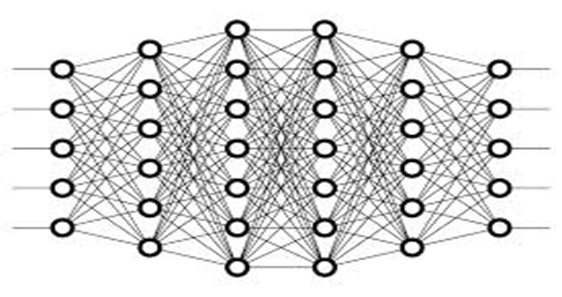
\includegraphics[width=0.8\textwidth]{My-Thesis/Chap1/images/lstm.png}
    \caption{Réseau de neurone complexe.}
    \label{fig:lstm_sequence}
\end{figure}

\mySubSection{Limites du Deep Learning}{}
\mySubSubSection{Opacité des Modèles}{}
Les modèles de DL sont souvent qualifiés de « boîtes noires » en raison de leur complexité architecturale et du grand nombre de paramètres (parfois des millions) \cite{rudin2019stop}. Cette opacité rend difficile l’interprétation des décisions, ce qui pose problème dans le contrôle d’accès, où les administrateurs doivent justifier les refus ou les autorisations d’accès. Cette sous-section explore les raisons techniques de cette opacité, comme la non-linéarité des fonctions d’activation et l’interdépendance des couches, et leurs implications pour la confiance des utilisateurs \cite{jouis2020}.

\mySubSubSection{Biais et Discriminations}{}
Les modèles de DL peuvent hériter ou amplifier des biais présents dans les données d’entraînement, entraînant des décisions discriminatoires, comme le refus d’accès basé sur des corrélations démographiques non pertinentes \cite{slack2020fooling}. Cette partie examine les sources de biais (données déséquilibrées, étiquettes erronées) et leur impact dans le contrôle d’accès, ainsi que les défis pour les détecter et les corriger sans outils d’explicabilité adaptés.

\mySubSubSection{Conformité aux Réglementations}{}
Les réglementations, comme l’article 22 du RGPD, exigent que les décisions automatisées soient accompagnées d’explications compréhensibles \cite{goodman2017gdpr}. Cette sous-section analyse les obstacles à la production d’explications conformes avec les modèles de DL, en raison de leur complexité et de l’absence de méthodes d’explicabilité standardisées. Elle discute des implications pour les systèmes de contrôle d’accès, où la conformité est cruciale \cite{desmoulin2019}.

% \begin{figure}[h]
%     \centering
%     \includegraphics[width=0.8\textwidth]{bias_visualization.png}
%     \caption{Représentation des biais dans un modèle de DL pour le contrôle d’accès, montrant comment des corrélations non pertinentes (par exemple, démographiques) peuvent influencer une décision de refus d’accès. Cette visualisation met en évidence la nécessité d’outils d’explicabilité pour détecter ces biais.}
%     \label{fig:bias_visualization}
% \end{figure}

\mySubSection{Nécessité de l’Explicabilité}{}
Face aux limites du DL, l’\textit{Explainable Artificial Intelligence} (XAI) émerge comme une solution pour rendre les modèles plus transparents et conformes. Cette section introduit les principales méthodes d’explicabilité, telles que LIME (approximation linéaire locale), SHAP (valeurs de Shapley), et les mécanismes d’attention, qui permettent de justifier les décisions des modèles \cite{ribeiro2016lime, lundberg2017shap, lin2017structured}. Elle souligne leur pertinence pour le contrôle d’accès, où les explications doivent être à la fois précises, compréhensibles, et conformes aux exigences légales \cite{barredo2020xai}. Une discussion sur l’équilibre entre performance et explicabilité conclut cette partie.

\mySubSection{Conclusion de la Section}{}
Cette section a exploré les principes fondamentaux, les applications, et les limites de l’apprentissage profond, en mettant l’accent sur son rôle dans le contrôle d’accès. Si le DL offre une puissance et une flexibilité inégalées, son opacité, ses biais potentiels, et les défis de conformité réglementaire nécessitent des approches d’explicabilité robustes. Ces concepts préparent le terrain pour les sections suivantes, qui analyseront les méthodes d’explicabilité et les systèmes de contrôle d’accès traditionnels et basés sur l’IA.
